\section{Quantum states}

The collection of all the information which one possesses about a quantum system identifies a \textit{quantum state}. 

\subsubsection{Pure states}

A quantum system can be described by \textit{pure states} $\ket{\psi}$ which are vectors of a Hilbert space $\mathcal{H}$ defined on a complex field:
\begin{align*}
    \ket{\psi}, ~\ket{\phi} \in \mathcal{H} \quad & \implies \quad \ket{\psi} + \ket{\phi} \in \mathcal{H}, \\ 
    \ket{\psi} \in \mathcal{H} \quad & \implies \quad \lambda \ket{\psi} \in \mathcal{H}, ~ \lambda \in \mathbb{C}.
\end{align*}
Moreover, $\ket{\psi}$ and $\lambda \ket{\psi}$ are the same state, but
\begin{align*}
    \lambda_1 \ket{\psi} + \lambda_2 \ket{\phi}  \quad  \text{and} \quad \lambda_2 \ket{\psi} + \lambda_1 \ket{\phi} 
\end{align*}
are not. 
\newline
The pure states are defined with a \textit{product scalar metric} (also called Hilbert metric), which for two generic elements $\ket{\psi}$ and $\ket{\phi} \in \mathcal{H}$, is given by the bra-ket of them:
\begin{align*}
    \braket{\psi}{\phi} = \braket{\phi}{\psi}^*.
\end{align*}
This quantity represents the projection of the state $\ket{\phi}$ on the state $\ket{\psi}$ and it is possible to define the \textit{fidelity} as 
\begin{align*}
    P = \abs{\braket{\psi}{\phi}}^2 = \braket{\psi}{\phi} \braket{\phi}{\psi}.
\end{align*}
If the states are normalized to 1, it gives the probability of preparing $\ket{\phi}$ and then measuring $\ket{\psi}$. From these considerations follows that two states which are orthonormal (i.e. $\braket{\psi}{\phi} = 0$ ) are fully distinguishable. 
\newline
Finally, the name ``metric" is associated to the fact that it introduces the concept of ``distance" between states. 

\begin{tcolorbox}
The Bures metric (or Helstrom metric) is an example of metric in which the distance between two states is given by
\begin{align*}
    D_B(\psi, \phi) = \sqrt{2 (1 - \abs{\braket{\psi}{\phi}})}.
\end{align*}
\end{tcolorbox}

\subsubsection{Orthonormal bases}
A generic state vector can be expanded in any orthonormal basis $\{ \ket{n}\}$:
\begin{align}
\label{eq:exp_basis}
    \ket{\psi} = \sum_n \ket{n} \braket{n}{\psi} = \sum_n c_n \ket{n},
\end{align}
where $n$ is a generic label which contains one or more integers. Moreover, since the elements of the basis are orthonormal
\begin{align*}
    \braket{n}{n'} = \delta_{n,n'}. 
\end{align*}
A final note: the summation in (\ref{eq:exp_basis}) contains a finite number of terms because, for all practical purposes, the dimension of $\mathcal{H}$ is finite (or countable infinite) since the studied sample has a finite size and one works at bounded energies and bandwidth. 

\subsection{Superposition and interference}

Quantum mechanics allows for superpositions of states. For example, one possible normalized superposition of two orthogonal states $\ket{\psi_1}$ and $\ket{\psi_2}$ is 
\begin{align*}
    \ket{+} = \frac{\ket{\psi_1} + \ket{\psi_2}}{\sqrt{2}} 
\end{align*}
and the probability that a generic state $\ket{\varphi}$ is measured starting from $\ket{+}$ is 
\begin{align}
\label{eq:prob_sup}
    P_{ + \to \varphi } = \abs{\braket{\varphi}{+}}^2 = \frac{\abs{\braket{\varphi}{\psi_1} + \braket{\varphi}{\psi_2}}^2}{2} = \frac{\abs{c_1 + c_2}^2}{2} 
\end{align}
where $c_1 = \braket{\varphi}{\psi_1}$ and $c_2 = \braket{\varphi}{\psi_2}$ are called \textit{amplitudes}. It is important to notice that (\ref{eq:prob_sup}) is different from the sum of the two amplitudes squared. 

Quantum interference is associated to the fact that an individual particle, such as a photon, can cross its own trajectory and interfere with the direction of its path. Moreover, it can also happen that the intervention from noise in the environment damages the quantum object and the wavefunctions of particles can either reinforce or diminish each other.



\section{Observables and measurements}

\subsection{Observables and operators}

Observables in quantum mechanics are associated with a self-adjoint linear operator (or with a Hermitian operator in the finite-dimensional case) acting on states of the Hilbert space $\mathcal{H}$. Consider a Hermitian operator $\hat{A}$ (i.e. such that $\hat{A} = \hat{A}^\dagger$) and any two states $\ket{\psi_1}$ and $\ket{\psi_1}$ in $\mathcal{H}$, then 
\begin{align*}
    \bra{\psi_1} \hat{A} \ket{\psi_2} &\equiv \left(\psi_1, \hat{A} \psi_2 \right)_\mathcal{H} \\
    &= \left(\hat{A}^{\dagger} \psi_1, \psi_2 \right)_\mathcal{H} \\ 
    &= \left(\psi_2, \hat{A}^{\dagger} \psi_1 \right)^*_\mathcal{H} \equiv  \left(\bra{\psi_2} \hat{A}^{\dagger} \ket{\psi_1} \right)^*,
\end{align*}
where the definition of Hermitian conjugate is used to pass from the first to the second line. 

\subsubsection{Expectation values}

The expectation value of the observable $\hat{A}$ when the system is in state $\ket{\psi}$ is
\begin{align*}
    \langle \hat{A} \rangle \equiv \bra{\psi} \hat{A} \ket{\psi}. 
\end{align*}


\subsubsection{Diagonal operators}

According to the Spectral Theorem, for a given Hermitian matrix $A$ (associated to the operator $\hat{A}$), there exists an orthonormal basis consisting of eigenvectors of $A$ which allows to diagonalize it. In addition, the eigenvalues are real. Therefore, it is always possible to find a transformation described by the matrix $U$ for which is valid
\begin{align}
    \label{eq:diago}
    A = U D \, U^\dagger, 
\end{align}
where $U$ is such that ${U} {U}^\dagger = {U}^\dagger {U} = \mathbb{I}$ (unitary matrix) and $D$ is a diagonal matrix. After the transformation in (\ref{eq:diago}), the operator $\hat{A}$ can be written as 
\begin{align*}
    \hat{A} = \sum_j \eta_j \ket{\varphi_j} \bra{\varphi_j}, 
\end{align*}
with $\ket{\varphi_j}$ eigenvectors associated to the eigenvalues $\eta_j$ such that $\eta_j = \eta_j^*$. 
\newline

A final note about the notation: in the following pages, the hat symbol (\^{}) for the operator is often omitted.

\subsubsection{Commutation between operators}

In general, operators do no commute, i.e.
\begin{align*}
    i[A,B] = C. 
\end{align*}
Hence for $C \neq 0$ the operators $A$ and $B$ do not have the same eigenstates and eigenvalues. 

\subsubsection{Uncertainty principle}

Heisenberg's uncertainty principle states that for any two operators $A$ and $B$, one has 
\begin{align}
    \label{eq:unc_princ}
    \Delta A \, \Delta B ~\geq~ \frac{1}{2} \abs{\langle [A,B] \rangle}, 
\end{align}
where
\begin{align*}
    (\Delta A)^2 &= {\langle \left( A - \langle A \rangle \right)^2\rangle } = {\langle A^2 \rangle - \langle A \rangle^2} \\
    (\Delta B)^2 &= {\langle \left( B - \langle B \rangle \right)^2\rangle } = {\langle B^2 \rangle - \langle B \rangle^2} 
\end{align*}

\begin{tcolorbox}
Consider the following states 
\begin{align}
    \label{eq:bits}
    \ket{0} = \begin{pmatrix} 1 \\ 0 \end{pmatrix} \qquad \qquad \ket{1} = \begin{pmatrix} 0 \\ 1 \end{pmatrix} 
\end{align}
and operators (Pauli matrices)
\begin{align}
    \label{eq:Pauli_mat}
    \sigma^x = \begin{pmatrix} 0 & 1 \\ 1 & 0 \end{pmatrix} \qquad
    \sigma^y = \begin{pmatrix} 0 & -i \\ i & 0 \end{pmatrix} \qquad
    \sigma^z = \begin{pmatrix} 1 & 0 \\ 0 & -1 \end{pmatrix} 
\end{align}
and try to apply the Heisenberg's uncertainty principle to $\sigma^z$ and $\sigma^x$: 
\begin{align*}
    (\Delta \sigma^z_0)^2 &= \bra{0} \left(\sigma^z - \bra{0} \sigma^z \ket{0} \right)^2 \ket{0} = \bra{0} \left(\sigma^z - 1\right)^2 \ket{0} = 0 ~~(\text{infinite accuracy}) \\
    (\Delta \sigma^x_0)^2 &= \bra{0} \left(\sigma^x - \bra{0} \sigma^x \ket{0} \right)^2 \ket{0} = \bra{0} \left(\sigma^x\right)^2 \ket{0} = \braket{0}{0} = 1 ~~(\text{finite accuracy})
\end{align*}
By knowing that $[\sigma^z, \sigma^x] = 2 i \, \sigma^y$, from (\ref{eq:unc_princ}) one obtains $0 \geq 0$.
\end{tcolorbox}

\subsection{The measurement process}

Consider a pure state $\ket{\psi}$ and imagine to apply an operator $O$ associated to a given observable. This measurement procedure returns an element in the spectrum (set of eigenvalues) of the observable; if $\lambda$ is the outcome of the procedure, then $\lambda \in \text{Spec}\{O\}$. In this process, the initial state $\ket{\psi}$ collapse onto different one and this can be described by introducing the projector operator $\Pi_\lambda$. The latter allows to obtain the projection of the initial state onto the eigenvectors related to the eigenvalue $\lambda$ and it is such that $\Pi_\lambda = \Pi_\lambda^2 = \Pi_\lambda^\dagger$. Hence, the measurement procedure can be represented by
\begin{align}
    \label{eq:meas}
    O \, \Pi_\lambda \ket{\psi} = \Pi_\lambda \, O \ket{\psi} =  \Pi_\lambda \, \lambda \ket{\psi} = \lambda \,\Pi_\lambda \ket{\psi}. 
\end{align}
The first equation is valid because $[\Pi_\lambda, O] = 0$, while the final state after the measurement is indicated by $\Pi_\lambda \ket{\psi}$. Therefore
\begin{align*}
    \ket{\psi} ~~ \text{before measurement} ~~~\longrightarrow~~~ \frac{\Pi_\lambda \ket{\psi}}{ \abs{\bra{\psi} \Pi_\lambda \ket{\psi}}} ~~ \text{after measurement,}
\end{align*}
where the denominator on the right is added to obtain a normalized final state. 
\newline
The probability associated to the measurement of the eigenvalue $\lambda$ is
\begin{align}
    P_\lambda = \abs{\bra{\psi} \Pi_\lambda \ket{\psi}}^2, 
\end{align}
if the states are normalized. 

It is important to notice that this process breaks the time reversal symmetry. 

\subsection{Physical transformation of a quantum system}

A physical transformation changes the state of the system:
\begin{align*}
    \ket{\psi} ~~ \text{before transformation} ~~~\longrightarrow~~~  \ket{\psi'} = T \ket{\psi} \equiv \ket{T\psi} ~~ \text{after transformation.}
\end{align*}

If a system is \textit{closed} (the energy is conserved in time), under any physical transformation: 
\begin{itemize}
    \item it stays deterministic (no randomness is involved in the development of future states of the system);
    \item it preserves the total probability.
\end{itemize}
Given any two states $\ket{\psi}$ and $\ket{\varphi}$, it is possible to write
\begin{align}
    \label{eq:transf}
    \big({T \psi}, {T \varphi} \big)_\mathcal{H} = \big({\psi}, {\varphi} \big)_\mathcal{H} = \braket{\psi}{\varphi},
\end{align}
and, since the probability is conserved from the last statement, relation (\ref{eq:transf}) becomes
\begin{align}
    \big|{\big({T \psi}, {T \varphi} \big)_\mathcal{H} } \big| = \big|{\big({\psi}, {\varphi} \big)_\mathcal{H}} \big|
\end{align}
This result originates two possibilities:
\begin{enumerate}
    \item $T$ is \textit{antiunitary}, i.e.
    \begin{align*}
        \big({T \psi}, {T \varphi} \big)_\mathcal{H} = \big( {\psi}, {\varphi} \big)_\mathcal{H}^*.
    \end{align*}
    Antiunitary operators are important in quantum theory because they are used to represent certain symmetries, such as time reversal.
    \item $T$ is \textit{unitary}, i.e.
    \begin{align*}
        \big({T \psi}, {T \varphi} \big)_\mathcal{H} = \big( {\psi}, {\varphi} \big)_\mathcal{H}.
    \end{align*}
   There is an equivalent definition: an operator T is unitary if $T^\dagger T = T T^\dagger = \mathbb{I}$. In addition, the product of two unitary operators is still unitary. The time evolution operators presented in the following are of this type. 
\end{enumerate}

\section{Time evolution of a quantum system}

Consider the evolution of a pure closed system; at the initial time $t_0$, the system is described by the state $\ket{\psi(t_0)} = \ket{\psi_0}$ and it is possible to evaluate the expectation value of a given operator $O$ at different times: $\langle O \rangle_{t_0}$, $\langle O \rangle_{t_1}$, ...,  $\langle O \rangle_{t_n}$ in order to characterize the evolution. For a generic quantity $\langle O \rangle_t \equiv \bra{\psi} O \ket{\psi}_t$, there are two possibilities: 
\begin{itemize}
    \item to consider to evolution of the state $\ket{\psi}$:
    \begin{align*}
        \bra{\psi} O \ket{\psi}_t = \bra{\psi(t)} O \ket{\psi(t)} \qquad \longrightarrow \qquad \text{Schr\"odinger picture;}
    \end{align*}
    \item to consider the evolution of the operator $O$:
    \begin{align*}
        \bra{\psi} O \ket{\psi}_t = \bra{\psi_{t_0}} O(t) \ket{\psi_{t_0}} \qquad \longrightarrow \qquad \text{Heisenberg picture.}
    \end{align*}
\end{itemize}

\subsection{Schr\"odinger picture}

In the Schr\"odinger picture the states are functions of time and the Schr\"odinger equation holds for every quantum system evolution that is physical, closed and first-order differential in time. The Hamiltonian is time-independent and the formal solutions are obtained in the following way:
\begin{enumerate}
    \item diagonalization of the Hamiltonian $H = \sum_j \varepsilon_j \ket{\varepsilon_j}\bra{\varepsilon_j}$ in order to write the time evolution in the form 
    \begin{align*}
        \ket{\varepsilon_j} \longrightarrow e^{-i \varepsilon_j t / \hbar} \ket{\varepsilon_j};
    \end{align*}
    \item expansion of the initial state $\ket{\psi_0}$ in the eigenbasis $\ket{\psi_0} = \sum_j c_j \ket{\varepsilon_j}$ and evolved state $\ket{\psi(t)} = \sum_j c_j \ket{\varepsilon_j} e^{-i \varepsilon_j t / \hbar}$ with $c_j = \braket{\varepsilon_j}{\psi_0}$; 
    \item expression of the evolved state with the matrix exponential
    \begin{align*}
        \ket{\psi(t)} = \left( \sum_j c_j \ket{\varepsilon_j} e^{-i \varepsilon_j t / \hbar} \bra{\varepsilon_j} \right) \ket{\psi_0} = \exp{-\frac{i }{\hbar}Ht} \ket{\psi_0}. 
    \end{align*}
\end{enumerate}

\subsection{Heisenberg picture}

In the Heisenberg picture, the states are constant in time while the operators evolve; for instance the expectation value of an operator $O$ is 
\begin{align*}
    \langle O \rangle_t = \bra{\psi} O \ket{\psi}_t = \bra{\psi_0} U^\dagger(t) O U(t) \ket{\psi_0} = \bra{\psi_0} \Tilde{O}(t) \ket{\psi_0} 
\end{align*}
and its evolution in time is 
\begin{align*}
    \frac{d}{dt} \Tilde{O}(t) &= \left(\frac{d}{dt} U^\dagger(t)\right) \, O \, U(t) + U^\dagger(t) \, O \, \left( \frac{d}{dt} U(t) \right) = \\
    &= \frac{i}{\hbar} H(t) U^\dagger(t) \, O \, U(t) - \frac{i}{\hbar}U^\dagger(t) \, O \, U(t) H(t) = \\
    &= \frac{i}{\hbar} H(t) \Tilde{O}(t) - \frac{i}{\hbar} \Tilde{O}(t) H(t) = \\
    &= \frac{i}{\hbar} [H(t), \Tilde{O}(t)].
\end{align*}
The last equation is called Heisenberg equation. 


\begin{tcolorbox}[breakable, enhanced]
\textbf{Driven two-level system} \\
Consider a system described by the Hamiltonian 
\begin{align*}
    H = \hbar \left( \Omega \sigma^x + \Delta \sigma^z \right),
\end{align*}
where $\sigma^x$ and $\sigma^z$ are the Pauli matrices in (\ref{eq:Pauli_mat}); therefore, 
\begin{align*}
    H = \hbar \begin{pmatrix} \Delta & \Omega \\ \Omega & -\Delta \end{pmatrix}.
\end{align*}
The eigenvalues are $\pm \sqrt{\Omega^2 + \Delta^2}$ and hence the energy difference between the two levels is $2 \sqrt{\Omega^2 + \Delta^2}$. This Hamiltonian can be rewritten by introducing 
\begin{align*}
    \Tilde{\Omega} = \sqrt{\Omega^2 + \Delta^2} \qquad \qquad \theta = \arctan{\left( \frac{\Delta}{\Omega} \right)}, 
\end{align*}
and 
\begin{align*}
    \Vec{n} = \begin{pmatrix} \cos{\theta} \\ 0 \\ \sin{\theta} \end{pmatrix} \qquad \qquad 
    \Vec{\sigma} = \begin{pmatrix} \sigma^x \\ \sigma^y \\ \sigma^z \end{pmatrix}
\end{align*}
from which 
\begin{align*}
    \Omega = \Tilde{\Omega} \cos{\theta}, \qquad \qquad \Delta = \Tilde{\Omega} \sin{\theta} \qquad \implies \qquad H = \hbar \Tilde{\Omega} \left( \Vec{n} \cdot \Vec{\sigma} \right). 
\end{align*}
Therefore the evolution operator becomes 
\begin{align*}
    \exp{ -i\frac{Ht}{\hbar}} &= \sum_j \frac{(-i \Tilde{\Omega} t)^j}{j!} \left( \Vec{n} \cdot \Vec{\sigma} \right)^j = \\
    &= \mathbb{I} \sum_{j ~ \text{even}} \frac{(-i \Tilde{\Omega} t)^j}{j!} + \left( \Vec{n} \cdot \Vec{\sigma} \right) \sum_{j ~\text{odd}} \frac{(-i \Tilde{\Omega} t)^j}{j!} = \\
    &= \mathbb{I} \cos{(\Tilde{\Omega}t)} + \left( \Vec{n} \cdot \Vec{\sigma} \right) (-i \sin{(\Tilde{\Omega}t)}) = \\
    &= \mathbb{I} \cos{(\Tilde{\Omega}t)} + \left( \sin{\theta} \sigma^z + \cos{\theta} \sigma^x \right) (-i \sin{(\Tilde{\Omega}t})) = \\
    &= \cos{(\Tilde{\Omega}t)}  \begin{pmatrix} 1 & 0 \\ 0 & 1 \end{pmatrix} - i \sin{(\Tilde{\Omega}t)} \begin{pmatrix} \sin{\theta} & \cos{\theta} \\ \cos{\theta} & -\sin{\theta} \end{pmatrix} 
\end{align*}
Now suppose to start from the state $\ket{\psi_0} = \ket{0}$ and study the evolution up to a time $t$. Form the previous expression for the evolution operator, it is straightforward to find 
\begin{align*}
    \ket{\psi(t)} = \cos{(\Tilde{\Omega}t)} \begin{pmatrix} 1 \\ 0 \end{pmatrix} - i \sin{(\Tilde{\Omega}t)}  \begin{pmatrix} \sin{\theta} \\ \cos{\theta} \end{pmatrix}. 
\end{align*}
Now, the expression for the probability of having the state $\ket{1}$ starting from the state $\ket{0}$ after a time $t$ is given by 
\begin{align*}
    P_{0 \to 1}(t) = \abs{\braket{1}{\psi(t)}}^2 = \abs{\begin{pmatrix} 0 & 1 \end{pmatrix} \begin{pmatrix}  \cos{(\Tilde{\Omega}t)} - i \sin{(\Tilde{\Omega}t)} \sin{\theta} \\ -i \sin{(\Tilde{\Omega}t)} \cos{\theta} \end{pmatrix}}^2 = \sin^2(\Tilde{\Omega}t) \cos^2{\theta}.
\end{align*}
It is important to notice that this probability oscillates with time and never reaches 1; indeed 
\begin{align*}
    P_{0 \to 1}^\text{max} = \cos^2{\theta} = \frac{\Omega^2}{\Omega^2 + \Delta^2} = 1 - \frac{\Delta^2}{\Omega^2 + \Delta^2}. 
\end{align*}
The only situation in which $P_{0 \to 1}^\text{max} \simeq 1$ is when $\Delta \ll
 \Omega$. In addition, it is possible to derive the oscillation period and the instants of time at which $P_{0 \to 1}^\text{max}$ is reached: 
\begin{align*}
    T = \frac{2 \pi}{2 \Tilde{\Omega}} \qquad \text{and} \qquad t_\text{max} = (2j+1) \frac{\pi}{2 \Tilde{\Omega}} \qquad \text{with} \qquad j \in \mathbb{Z}. 
\end{align*}
Obviously, the frequency associated to the energy gap between the states ($2\Tilde{\Omega}$) is the same obtained from the diagonalization of the initial Hamiltonian. A note about this: the highest frequency at which this system can oscillate is the one associated to the largest energy gap between the level, hence $2\Tilde{\Omega}$. \\

A pictorial view of the system with the Bloch sphere is reported in figure \ref{fig:Bloch_sphere}.
\end{tcolorbox}

\begin{figure}[H]
\centering
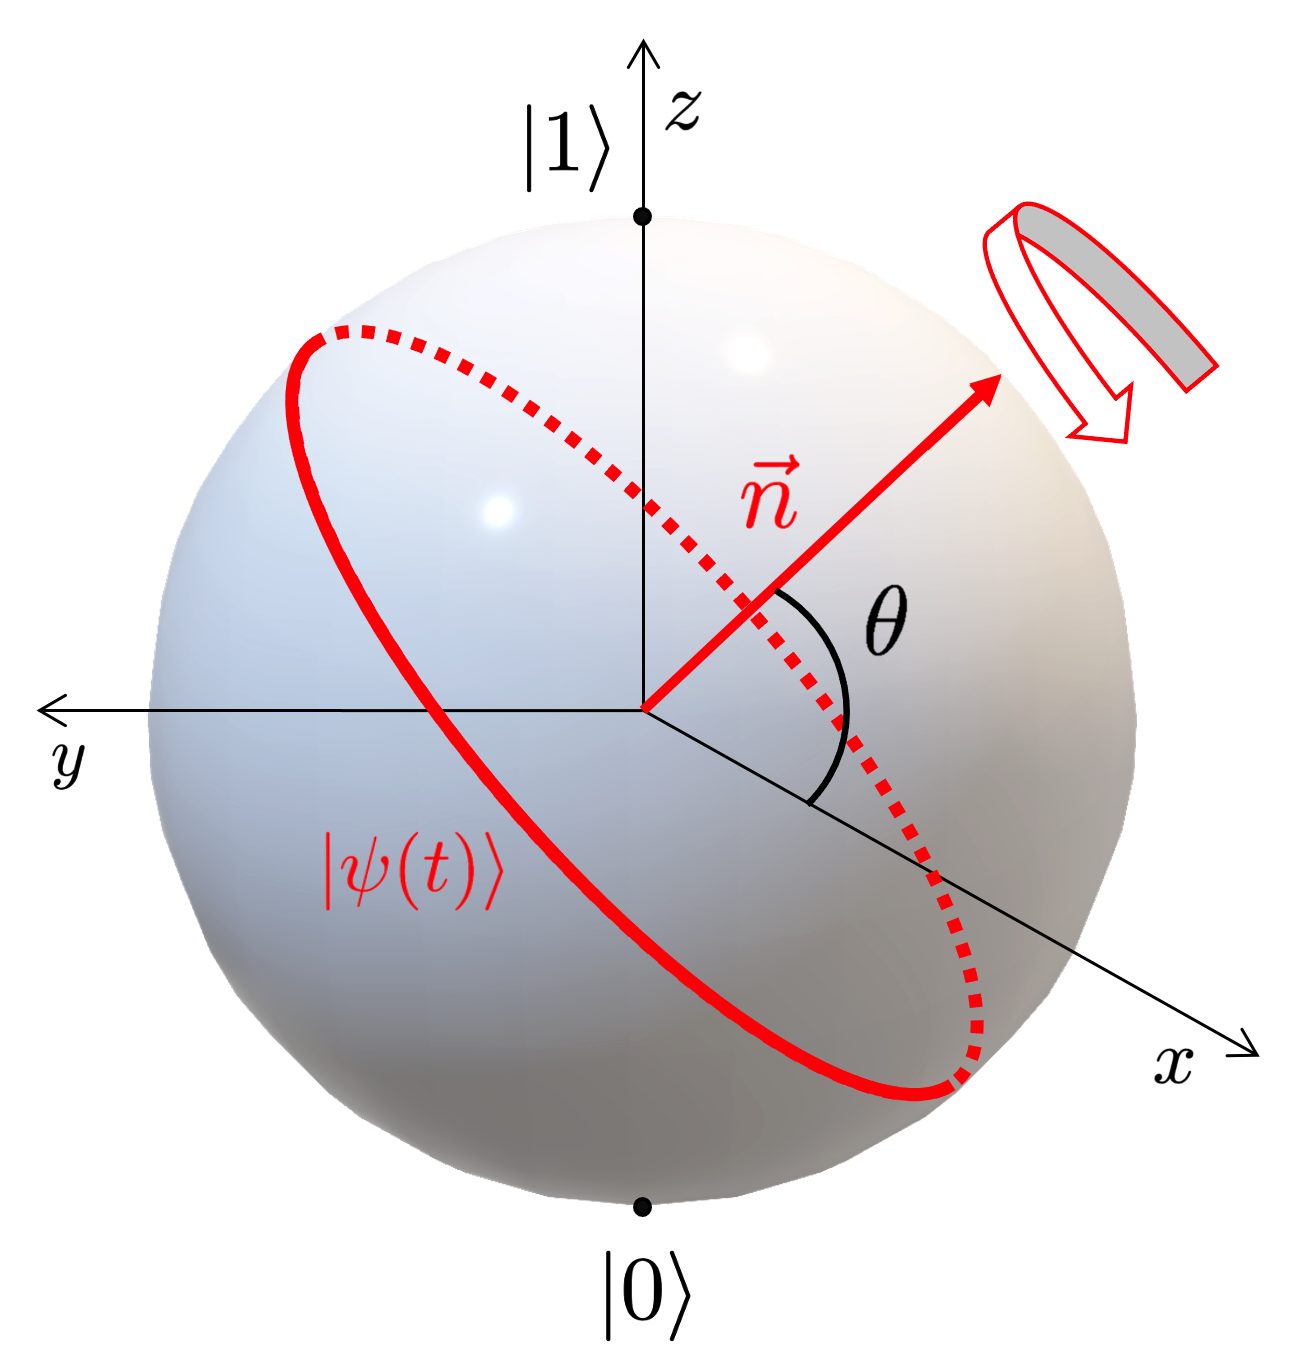
\includegraphics[width=0.42\linewidth]{images/Driven_two-level_system.png}
    \caption{Scheme of a driven two-level system with the Bloch sphere. The state $\ket{\psi(t)}$ is on the red circumference and it rotates with frequency $2 \Tilde{\Omega}$ around the vector $\Vec{n}$.}
    \label{fig:Bloch_sphere}
\end{figure}

\section{Time-independent degenerate perturbation theory}
\label{sec:timedep}

Consider a system described by the time-independent Hamiltonian $H = H_0 + \lambda V$, where $\lambda V$ is a perturbation (small when $\lambda \to 0$) and $H_0$ is the unperturbed Hamiltonian. The latter has eigenstates obtained by solving the eigenvalue equation: 
\begin{align*}
    H_0 \ket{\varepsilon^{(0)}_n, J} = \varepsilon^{(0)}_n \ket{\varepsilon^{(0)}_n, J}, 
\end{align*}
where $J$ is an index introduced to take into account the degeneracy of the states. 
The eigenvalue equation for the perturbed system is instead: 
\begin{align}
    \label{eq:SchEq_pert}
    (H_0 + \lambda V) \ket{\Tilde{\varepsilon}_n,J}= \Tilde{\varepsilon}_n \ket{\Tilde{\varepsilon}_n,J}, 
\end{align}
If $\lambda$ is small, $\ket{\Tilde{\varepsilon}_n}$ and $\Tilde{\varepsilon}_n$ can be written as a series expansion which takes into account the corrections to $\ket{\varepsilon^{(0)}_n}$ and $\varepsilon^{(0)}_n$:
\begin{align*}
    \Tilde{\varepsilon}_n &= \varepsilon^{(0)}_n + \lambda \varepsilon^{(1)}_n + \lambda^2 \varepsilon^{(2)}_n + ... \\
    \ket{\Tilde{\varepsilon}_n,J} &= \ket{\varepsilon^{(0)}_n,J_0} + \lambda \ket{\varepsilon^{(1)}_n,J_1} + \lambda^2 \ket{\varepsilon^{(2)}_n,J_2} + ...
\end{align*}
Inserting these expressions at first order in (\ref{eq:SchEq_pert})
\begin{align*}
    (H_0 + \lambda V) \left(\ket{\varepsilon^{(0)}_n,J_0} + \lambda \ket{\varepsilon^{(1)}_n,J_1} \right) = \left( \varepsilon^{(0)}_n + \lambda \varepsilon^{(1)}_n \right)\left(\ket{\varepsilon^{(0)}_n,J_0} + \lambda \ket{\varepsilon^{(1)}_n,J_1} \right)
\end{align*}
and considering only the terms at the same order in $\lambda$, it is possible to find the corrections to the unperturbed values. The zeroth order is trivial, while the first order gives:
\begin{align}
    \label{eq:fo_pert1}
    V \ket{\varepsilon^{(0)}_n,J_0} + H_0 \ket{\varepsilon^{(1)}_n,J_1} = \varepsilon^{(1)}_n \ket{\varepsilon^{(0)}_n,J_0} + \varepsilon^{(0)}_n \ket{\varepsilon^{(1)}_n,J_1}
\end{align}
Now it is useful to introduce the projector onto the $\varepsilon^{(0)}_n$ eigenspace of $H_0$
\begin{align*}
    \Pi_{\varepsilon^{(0)}_n} = \sum_{J} \ket{\varepsilon^{(0)}_n, J} \bra{\varepsilon^{(0)}_n, J}
\end{align*}
and to multiply it to the left in equation (\ref{eq:fo_pert1}): 
\begin{align*}
    \Pi_{\varepsilon^{(0)}_n} V \ket{\varepsilon^{(0)}_n,J_0} + \Pi_{\varepsilon^{(0)}_n} H_0 \ket{\varepsilon^{(1)}_n,J_1} &= \varepsilon^{(1)}_n \Pi_{\varepsilon^{(0)}_n} \ket{\varepsilon^{(0)}_n,J_0} + \varepsilon^{(0)}_n \Pi_{\varepsilon^{(0)}_n} \ket{\varepsilon^{(1)}_n,J_1} \\
     \Pi_{\varepsilon^{(0)}_n} V \ket{\varepsilon^{(0)}_n,J_0} +  H_0 \Pi_{\varepsilon^{(0)}_n} \ket{\varepsilon^{(1)}_n,J_1} &= \varepsilon^{(1)}_n  \ket{\varepsilon^{(0)}_n,J_0} + \varepsilon^{(0)}_n \Pi_{\varepsilon^{(0)}_n} \ket{\varepsilon^{(1)}_n,J_1} \\
      \Pi_{\varepsilon^{(0)}_n} V \ket{\varepsilon^{(0)}_n,J_0} +  \cancel{\varepsilon^{(0)}_n \Pi_{\varepsilon^{(0)}_n} \ket{\varepsilon^{(1)}_n,J_1}} &= \varepsilon^{(1)}_n  \ket{\varepsilon^{(0)}_n,J_0} + \cancel{\varepsilon^{(0)}_n \Pi_{\varepsilon^{(0)}_n} \ket{\varepsilon^{(1)}_n,J_1}},
\end{align*}
where the fact that $ \Pi_{\varepsilon^{(0)}_n} H_0 = H_0 \Pi_{\varepsilon^{(0)}_n} =\varepsilon^{(0)}_n \Pi_{\varepsilon^{(0)}_n}$ is used. The last result obtained can be written as
\begin{equation}
    \label{eq:fo_pert2}
    \left( \Pi_{\varepsilon^{(0)}_n} V \Pi_{\varepsilon^{(0)}_n} \right) \ket{\varepsilon^{(0)}_n,J_0} = \varepsilon^{(1)}_n  \ket{\varepsilon^{(0)}_n,J_0} \qquad \forall J_0,
\end{equation}
since $\ket{\varepsilon^{(0)}_n,J_0} = \Pi_{\varepsilon^{(0)}_n} \ket{\varepsilon^{(0)}_n,J_0}$. The operator in brackets is called $H^{(1)} \equiv \Pi_{\varepsilon^{(0)}_n} V \Pi_{\varepsilon^{(0)}_n}$ and it is Hermitian, while equation (\ref{eq:fo_pert2}) is an eigenvalue equation. It states that the degeneracy is removed (since now the eigenstate of the unperturbed Hamiltonian is associated to an eigenvalue different from $\varepsilon^{(0)}_n$) and how the resolved states looks like. Moreover, it is important to notice that the resolved states are not a small correction from an arbitrary unperturbed state. 

\subsubsection{Higher orders of degeneracy-removing Hamiltonians}

With an approach similar to the one presented previously, it is possible to obtain the higher order Hamiltonians. Explicitly, up to the forth order, they are:
\begin{align}
    H^{(0)} =&~ H_0 \label{eq:H0} \\
    H^{(1)} =&~ \Pi_{\varepsilon^{(0)}_n} V \Pi_{\varepsilon^{(0)}_n} \label{eq:H1}\\
    H^{(2)} =&~\Pi_{\varepsilon^{(0)}_n} V R_{\varepsilon^{(0)}_n} V \Pi_{\varepsilon^{(0)}_n}  \label{eq:H2} \\
    H^{(3)} =&~ \Pi_{\varepsilon^{(0)}_n} V R_{\varepsilon^{(0)}_n} V R_{\varepsilon^{(0)}_n} V \Pi_{\varepsilon^{(0)}_n} + \nonumber \\
    &- \Pi_{\varepsilon^{(0)}_n} V \Pi_{\varepsilon^{(0)}_n} V R_{\varepsilon^{(0)}_n}^2 V \Pi_{\varepsilon^{(0)}_n} \label{eq:H3} \\
    H^{(4)} =&~ \Pi_{\varepsilon^{(0)}_n} V R_{\varepsilon^{(0)}_n} V R_{\varepsilon^{(0)}_n} V R_{\varepsilon^{(0)}_n} V \Pi_{\varepsilon^{(0)}_n} + \nonumber \\
    & -\Pi_{\varepsilon^{(0)}_n} V R_{\varepsilon^{(0)}_n}^2 V \Pi_{\varepsilon^{(0)}_n} V R_{\varepsilon^{(0)}_n} V \Pi_{\varepsilon^{(0)}_n} + \nonumber \\
    &- \Pi_{\varepsilon^{(0)}_n} V \Pi_{\varepsilon^{(0)}_n} V R_{\varepsilon^{(0)}_n} V R_{\varepsilon^{(0)}_n}^2 V \Pi_{\varepsilon^{(0)}_n} + \nonumber \\
    &+ \Pi_{\varepsilon^{(0)}_n} V \Pi_{\varepsilon^{(0)}_n} V R_{\varepsilon^{(0)}_n}^2 V R_{\varepsilon^{(0)}_n} V \Pi_{\varepsilon^{(0)}_n} + \nonumber \\
    &+ \Pi_{\varepsilon^{(0)}_n} V \Pi_{\varepsilon^{(0)}_n} V \Pi_{\varepsilon^{(0)}_n} V R_{\varepsilon^{(0)}_n}^3 V \Pi_{\varepsilon^{(0)}_n} \label{eq:H4}
\end{align}
In these expressions, the \textit{Moore-Penrose pseudoinverse} $R_{\varepsilon^{(0)}_n}$ is introduced and it is defined as:
\begin{equation}
    R_{\varepsilon^{(0)}_n} = \left(\varepsilon^{(0)}_n \mathbb{I} - H_0 \right)^{``-1"}.
\end{equation}

The higher order degeneracy-removing Hamiltonians are applied to an important system in order to see explicitly their effect on the energy levels and on the states. 

\begin{tcolorbox}[breakable, enhanced]
\textbf{The three-level system ($\Lambda$ system) with perturbation theory} \\
Consider a system with three states
\begin{align*}
    \ket{0} = \begin{pmatrix} 1 \\ 0 \\ 0 \end{pmatrix}, \qquad \qquad \ket{e} = \begin{pmatrix} 0 \\ 1 \\ 0 \end{pmatrix} \qquad \text{and} \qquad \ket{1} = \begin{pmatrix} 0 \\ 0 \\ 1 \end{pmatrix},
\end{align*}
and with unperturbed Hamiltonian given by 
\begin{align*}
    H_0 = \begin{pmatrix} 0 & 0 & 0 \\ 0 & \Delta & 0 \\ 0 & 0 & 0 \end{pmatrix}.
\end{align*}
This implies that the states $\ket{0}$ and $\ket{1}$ are degenerate with energy $\varepsilon_1^{(0)} = \varepsilon_2^{(0)} = 0$, while the state $\ket{e}$ has energy $\epsilon_3^{(0)} = \Delta$. Consider now a small perturbation described by the term
\begin{align*}
    V = \begin{pmatrix} 0 & \Omega & 0 \\ \Omega & 0 & \Omega \\ 0 & \Omega & 0 \end{pmatrix} = \Omega \begin{pmatrix} 0 & 1 & 0 \\ 1 & 0 & 1 \\ 0 & 1 & 0 \end{pmatrix}. 
\end{align*}
The first two orders of degeneracy-removing Hamiltonians can be found considering the projectors and the Moore-Penrose pseudoinverse matrices
\begin{align*}
    \Pi_0 &= \begin{pmatrix} 1 & 0 & 0 \\ 0 & 0 & 0 \\ 0 & 0 & 1 \end{pmatrix} \qquad
    R_0 = \begin{pmatrix} 0 & 0 & 0 \\ 0 & -1/\Delta & 0 \\ 0 & 0 & 0 \end{pmatrix} \\ \Pi_\Delta &= \begin{pmatrix} 0 & 0 & 0 \\ 0 & 1 & 0 \\ 0 & 0 & 0 \end{pmatrix} 
    \qquad R_\Delta = \begin{pmatrix} 1/\Delta & 0 & 0 \\ 0 & 0 & 0 \\ 0 & 0 & 1/\Delta \end{pmatrix} 
\end{align*}
and inserting them in (\ref{eq:H1}) and (\ref{eq:H2}):
\begin{align*}
    H^{(1)}_0 &= \Pi_0 V \Pi_0 = 0 \\
    H^{(1)}_\Delta &= \Pi_\Delta V \Pi_\Delta = 0  \\
    H^{(2)}_0 &= \Pi_0 V R_0 V \Pi_0 = -\frac{\Omega^2}{\Delta} \begin{pmatrix} 1 & 0 & 1 \\ 0 & 1 & 0 \\ 1 & 0 & 1 \end{pmatrix} \\
    H^{(2)}_\Delta &= \Pi_\Delta V R_\Delta V \Pi_\Delta = \frac{2 \Omega^2}{\Delta} \begin{pmatrix} 0 & 0 & 0 \\ 0 & 1 & 0 \\ 0 & 0 & 0 \end{pmatrix} \label{eq:H_Delta}
\end{align*}
The matrix $H^{(2)}_0$ can be diagonalized in order to find the new eigenvalues after the perturbation; they are
\begin{align*}
    \varepsilon^{(2)}_a = -\frac{2 \Omega^2}{\Delta} \qquad \text{and} \qquad \varepsilon^{(2)}_b = 0.
\end{align*}
It is possible to notice that the last state is transparent to the perturbation ($\varepsilon_2^{(2)} = 0$) and it is called \textit{dark state}. The other state is shifted to a lower energy equal to $\varepsilon_1^{(2)} = -2 \Omega^2/\Delta$.

The matrix $H^{(2)}_\Delta$ is already diagonalized and from it is evident that the energy of the initial excited state $\ket{e}$ increases of $2 \Omega^2/\Delta$; therefore, $\varepsilon_3^{(2)} = \Delta\left( 1 + {2 \Omega^2}/{\Delta^2}\right)$. Obviously, these corrections are negligible if $\Omega \ll \Delta$ and hence if the perturbation is small.
\\

A scheme of the system without and with the perturbation is reported in figure \ref{fig:lambda_sys}. 
\end{tcolorbox}

The same results can be obtained with a conventional approach without the perturbation theory. 

\begin{tcolorbox}[breakable, enhanced]
\textbf{The $\Lambda$ system without perturbation theory} \\
Now the same system of the previous example is studied without applying perturbation theory. The total Hamiltonian can be written as 
\begin{align*}
    H = \Delta \begin{pmatrix} 0 & \eta & 0 \\ \eta & 1 & \eta \\ 0 & \eta & 0 \end{pmatrix} \qquad \text{with} \qquad \eta = \frac{\Omega}{\Delta}.
\end{align*}

The eigenvalues are obtained diagonalizing the matrix:
\begin{align*}
    p(\alpha) &= \alpha^2 (1-\alpha) + 2 \alpha \eta^2 = -\alpha (\alpha^2 - \alpha - 2 \eta^2) \\
    p(\alpha) &= 0 \quad \implies \quad \alpha = 0, ~~\alpha = \frac{1}{2} \left( 1 \pm \sqrt{1+ 8 \eta^2}\right).
\end{align*}
For small values of $\eta$, the eigenvalues are:
\begin{align*}
    \varepsilon_1 &\simeq \frac{\Delta}{2} -\frac{\Delta}{2}(1 + 4 \eta^2) = - \frac{2 \Omega^2}{\Delta} \\
    \varepsilon_2 &= 0 \\
    \varepsilon_3 &\simeq \frac{\Delta}{2} + \frac{\Delta}{2}(1 + 4 \eta^2) = \Delta\left( 1 + \frac{2 \Omega^2}{\Delta^2}\right).
\end{align*}
The results are consistent with the expressions for $\varepsilon_1^{(2)}$, $\varepsilon_2^{(2)}$ and $\varepsilon_3^{(2)}$ obtained in the previous example. 
\end{tcolorbox}

\begin{figure}[H]
\centering
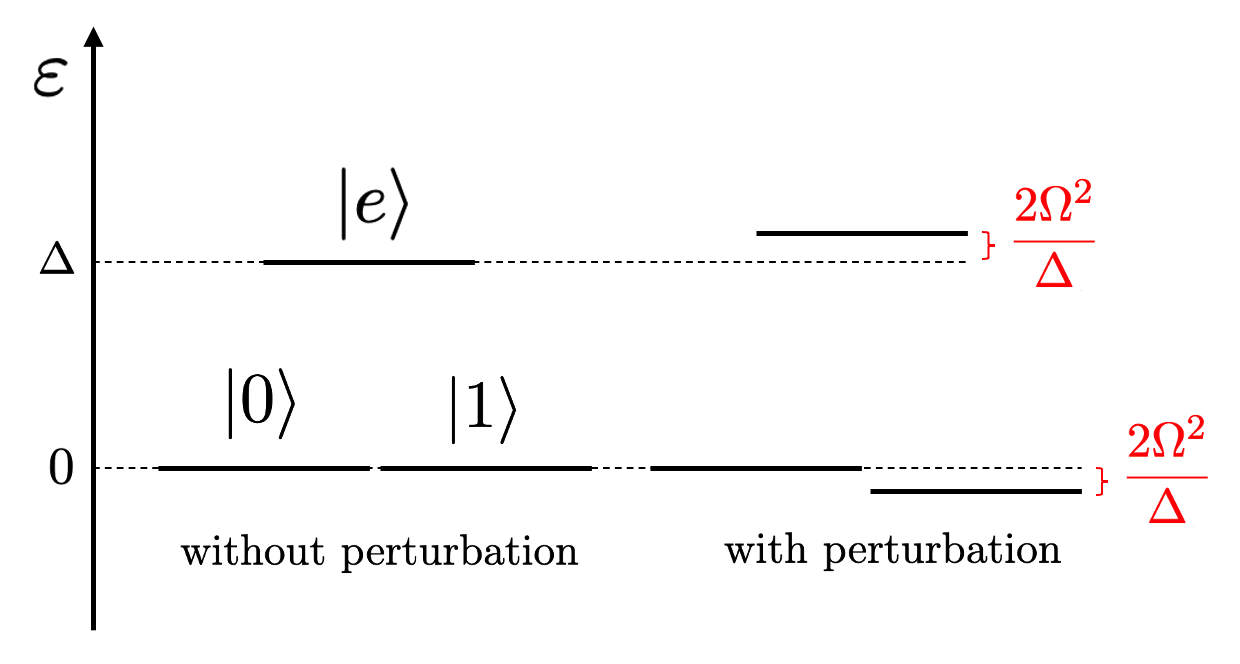
\includegraphics[width=0.66\linewidth]{images/Lambda_system.png}
    \caption{Scheme of a $\Lambda$ system without and with perturbation; it modifies the energy levels by removing the degeneracy and by increasing the separation between the ground states and the excited state.}
    \label{fig:lambda_sys}
\end{figure}

Some other considerations about the $\Lambda$ system can be done. First of all, the behaviour of the system for different values of the parameter $\Omega$ can be schematized as in figure \ref{fig:deg_rem}, where the degeneracy removal is evident. \\
Moreover, it is important to underline that it presents two typical energies (and hence two typical frequencies) $\Omega$ and $\Delta$ which can be associated to two characteristic motions of the system. The first one is related to the oscillations between the states $\ket{0}$ and $\ket{1}$ which happens with frequency $2 \Omega^2/\Delta$; it is named \textit{secular motion} because it is slow ($\Delta \gg \Omega$). The second one is related to the wiggles of the excited state $\ket{e}$ which are described by a frequency proportional to $\Delta$; it is named \textit{micromotion} because it is fast. 

\begin{figure}[t!]
\centering
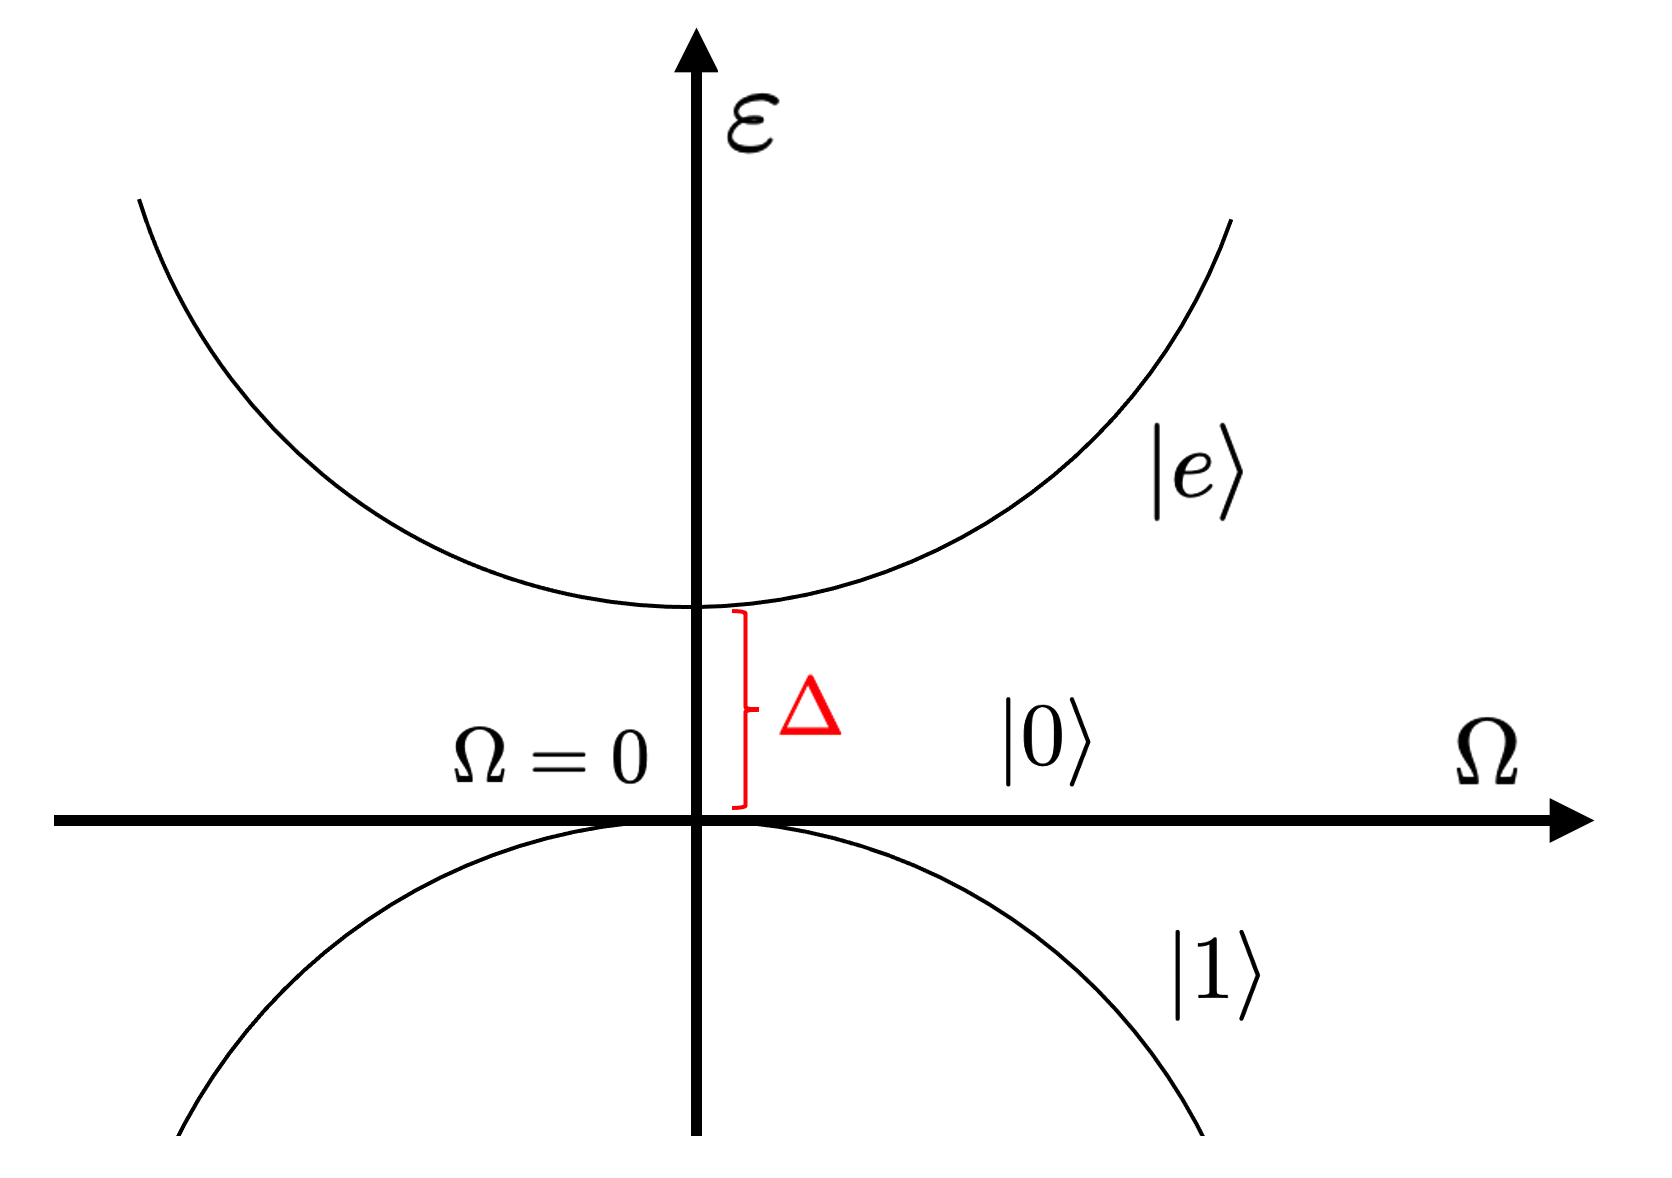
\includegraphics[width=0.61\linewidth]{images/Degeneracy_removal.png}
    \caption{Degeneracy removal in the $\Lambda$ system. For larger values of $\Omega$, the energy separation between the state $\ket{0}$ and the state $\ket{1}$ increases.}
    \label{fig:deg_rem}
\end{figure}

\section{Time-dependent Hamiltonians}
\label{sec:time_dep_sys}

\subsection{Time-ordered exponentials}

The Schr\"odinger equation with time-dependent Hamiltonian is 
\begin{equation}
    \label{eq:Schtime}
    i \hbar \frac{d}{dt}\ket{\psi(t)} = H(t)\ket{\psi(t)} \qquad \qquad \ket{\psi(t)} = U(t,t_0) \ket{\psi(t_0)}, 
\end{equation}
where $U$ is an unitary operator such that 
\begin{align*}
    U(t_2,t_1) U(t_1,t_0) = U(t_2,t_0) \qquad \text{additivity,} \\
    U(t,t) = \mathbb{I} \qquad \text{identity connection.}
\end{align*}
Equation (\ref{eq:Schtime}) can be rewritten in order to obtain an equation for $U(t,t_0)$:
\begin{equation}
    \label{eq:Utime}
    i \hbar \frac{dU}{dt} \cancel{\ket{\psi(t_0)}}= H(t) U(t,t_0) \cancel{\ket{\psi(t_0)}}.
\end{equation}
Consider now a small time increment $\delta t$ such that $U(t+\delta t,t_0)$ can be Taylor expanded
\begin{align*}
    U(t+\delta t,t_0) = U(t+\delta t,t) \, U(t,t_0) = U(t,t_0) + \delta t \frac{d U}{dt} + O(\delta t^2)
\end{align*}
and using equation (\ref{eq:Utime}) becomes 
\begin{align*}
    U(t+\delta t,t) \, \cancel{U(t,t_0)} = \cancel{U(t,t_0)} - \frac{i}{\hbar} \delta t \, H(t) \cancel{U(t,t_0)} + O(\delta t^2) \\
    U(t+\delta t,t) =\mathbb{I} - \frac{i}{\hbar} \delta t \, H(t) + O(\delta t^2) \simeq \exp{- \frac{i}{\hbar} \delta t \, H(t)}.
\end{align*}
The same calculations can be done for several infinitesimal time increments which allow to write $U(t,t_0)$ as 
\begin{align*}
    U(t,t_0) &= U(t,t-\delta t) \, U(t,t-2\delta t) \, ... \, U(t_0 + \delta t_0, t_0) \simeq \\
    &\simeq \exp{-\frac{i}{\hbar} \delta t \, H(t-\delta t)}  \exp{-\frac{i}{\hbar} \delta t \, H(t-2\delta t)} \, ... \, \exp{- \frac{i}{\hbar} \delta t \, H(t_0)} \overset{\delta t \to 0}{\equiv} \\
    &\overset{\delta t \to 0}{\equiv}  \mathcal{T}\exp{-\frac{i}{\hbar} \int_{t_0}^{t} H(t')dt'}. 
\end{align*}
The last lines are the definition of the \textit{time-ordered exponential} if $\delta t \to 0$; it is related to the well-known Dyson series which provide an analogous expression for $U(t,t_0)$. 
\begin{align*}
    U(t,t_0) = \mathbb{I} + \sum_{n=1}^\infty (-i)^n \int_{t_0}^{t} dt_1 \int_{t_0}^{t_1} dt_2 \, ... \, \int_{t_0}^{t_{n-1}} dt_n H(t_1) H(t_2) \, ... \, H(t_n)
\end{align*}

\subsection{Time-periodic system}
\label{subsec:1.5.2}
Consider the Hamiltonian 
\begin{equation}
    H(t) = H_0 + W(t),
\end{equation}
where $H_0$ describes the system and $W(t)$ is the external potential, also called \textit{drive}. By changing $H_0$ and $W(t)$ it is possible to control the system and to design some properties of it, but in general the solutions are not trivial. A simplified situation is the one in which the external potential is periodic: $W(t+T) = W(t)$; in this case, it is useful to study the \textit{time-averaged behaviour} of the system. 

The first step consists in writing the statevector $\ket{\psi(t)}$ in a new basis in order to introduce the state $\ket{\psi'(t)} = R(t) \ket{\psi(t)}$, where $R(t)$ is an unitary operator which therefore can be written as 
\begin{align*}
    R(t) = e^{i K(t)},
\end{align*}
where $K(t)$ is Hermitian. The Schr\"odinger equation for the system becomes 
\begin{align*}
    i \hbar \frac{d}{dt} \ket{\psi(t)} &= H(t)  \ket{\psi(t)} \\
    i \hbar \frac{d}{dt} \left( R^\dagger(t) \ket{\psi'(t)} \right) &= H(t) R^\dagger(t) \ket{\psi'(t)} \\
    i \hbar \, \frac{dR^\dagger(t)}{dt} \ket{\psi'(t)} + i \hbar \, R^\dagger(t) \frac{d}{dt} \ket{\psi'(t)} &= H(t) R^\dagger(t) \ket{\psi'(t)}.
\end{align*}
Multiplying by $R(t)$ on the left
\begin{align*}
    i \hbar \, R(t) \frac{dR^\dagger(t)}{dt} \ket{\psi'(t)} + i \hbar \,R(t) R^\dagger(t) \frac{d}{dt} \ket{\psi'(t)} &= R(t) H(t) R^\dagger(t) \ket{\psi'(t)}
\end{align*}
from which 
\begin{align*}
    i \hbar \frac{d}{dt} \ket{\psi'(t)} &= R(t) H(t) R^\dagger(t) \ket{\psi'(t)} - i \hbar R(t) \frac{dR^\dagger(t)}{dt} \ket{\psi'(t)} \\
    &= \left( R(t) H(t) R^\dagger(t) - i \hbar R(t) \frac{dR^\dagger(t)}{dt} \right) \ket{\psi'(t)}
\end{align*}
This is a Schr\"odinger equation for $\ket{\psi'(t)}$ with Hamiltonian 
\begin{align}
    H'(t) = R(t) H(t) R^\dagger(t) - i \hbar R(t) \frac{dR^\dagger(t)}{dt}. 
    \label{eq:transfH}
\end{align}
It is straightforward to show\footnote{The time-dependece is omitted in this proof.} that $H'(t)$ is Hermitian starting from
\begin{align*}
    H' &= R H R^\dagger - i \hbar R \frac{dR^\dagger}{dt} \\
    H'^\dagger &= R H^\dagger R^\dagger + i \hbar \left( \frac{d R^\dagger}{dt} \right)^\dagger R^\dagger = R H R^\dagger + i \hbar \frac{dR}{dt} R^\dagger
\end{align*}
and considering
\begin{align*}
    H'- H'^\dagger &= -i R \frac{d R^\dagger}{dt} - i \frac{d R}{dt} R^\dagger = \\
    &= -i\left( R \frac{d R^\dagger}{dt} + \frac{d R}{dt} R^\dagger \right) \\
    &= -i \frac{d}{dt} (R R^\dagger) = -i \frac{d \mathbb{I}}{dt} = 0. 
\end{align*}
Therefore,
\begin{align}
    \label{eq:Hprim}
    H'(t) = R(t) H(t) R^\dagger(t) - i \hbar R(t) \frac{dR^\dagger(t)}{dt} = R(t) H(t) R^\dagger(t) + i \hbar \frac{dR(t)}{dt} R^\dagger(t) 
\end{align}


It is interesting to notice that $H'(t)$ in (\ref{eq:Hprim}) can be built in such a way that it is time-independent ($H'(t) = H'$). The simplest way to achieve this condition is to start from a time-dependent Hamiltonian of the form
\begin{equation}
    \label{eq:start_ham}
    H(t) = H_0 + e^{i \omega t} V + e^{-i \omega t} V^\dagger,
\end{equation}
in which the periodic potential is monochromatic (fixed oscillation frequency) with $\omega \gg \Delta E/\hbar$ (\textit{high-frequency approximation}), where $\Delta E$ is the typical energy scale of $H_0$. In this case, assume that one can write the operators $H'$ and $K(t)$ in the general form
\begin{align*}
    H' = \sum_n \frac{1}{\omega^n} H'_n \qquad \text{and} \qquad
    K(t) = \sum_n \frac{1}{\omega^n} K_n(t);
\end{align*}
inserting these considerations in (\ref{eq:Hprim}), one can obtain
\begin{equation}
    \label{eq:final_ham}
    H' = H_0 + \frac{1}{\hbar \omega} [V,V^\dagger] + \frac{1}{2 (\hbar \omega)^2} \left( [[V,H_0],V^\dagger] + [[V^\dagger,H_0],V] \right) + O\left( \frac{1}{\omega^3} \right)
\end{equation}
in the case in which 
\begin{equation}
    \label{eq:K}
    K(t) = \frac{1}{i \hbar \omega } V e^{i \omega t} - \frac{1}{i \hbar \omega} V^\dagger e^{-i \omega t} + O \left( \frac{1}{\omega^2} \right). 
\end{equation}
It is important to underline that relations (\ref{eq:final_ham}) and (\ref{eq:K}) are approximated expressions which are valid only in the high-frequency regime, the most general relation for $H'(t)$ is (\ref{eq:Hprim}). Moreover, in this regime, it is possible to identify a fast dynamics (micro-motion) associated to the operator $K(t)$ and a slow dynamics (secular motion) associated to the operator $H'(t)$.

\begin{tcolorbox}[breakable, enhanced]
\textbf{Qubit system with a \textit{weak drive} in the high-frequency regime} \\
Consider the Hamiltonian of a two-level system
\begin{align}
    \label{eq:qubit_H0}
    H_0 = -J \sigma^x = -J \begin{pmatrix} 0 & 1 \\ 1 & 0 \end{pmatrix} 
\end{align}
and the periodic potential
\begin{align}
    \label{eq:qubit_W}
    W(t) = \Delta \cos{(\omega t)} \, \sigma^z = \frac{\Delta}{2} e^{i \omega t} \sigma^z + \frac{\Delta}{2} e^{-i \omega t} \sigma^z,
\end{align}
with $\hbar \omega \gg \Delta$ (weak drive) and $\hbar \omega \gg J$ (high-frequency regime). Notice that $H(t) = H_0 + W(t)$ is in the form (\ref{eq:start_ham}) and that there are three characteristic energies: $J$ (strength of the Hamiltonian), $\Delta$ (strength of the drive) and $\hbar \omega$ (energy of the drive oscillations); moreover, $V = V^\dagger = (\Delta/2) \sigma^z$ and $\omega \gg J/\hbar$ (high frequency regime). 
From (\ref{eq:final_ham}), the Hamiltonian in the new reference frame is made of two parts (at the second order approximation)
\begin{align*}
    H'= H_0 + \frac{1}{2 (\hbar \omega)^2} \, 2 \, [[V,H_0],V] = H_0 + \frac{1}{(\hbar \omega)^2}  [[V,H_0],V]  ,
\end{align*}
which can be explicitly computed:
\begin{align*}
    &[V,H_0] = \left[ \frac{\Delta}{2} \sigma^z, J \sigma^x \right] = -\frac{J\Delta}{2} [\sigma^z,\sigma^x] = - i J \Delta \sigma^y, \\
    &[[V,H_0],V] = \left[-i J \Delta \sigma^y, \frac{\Delta}{2} \sigma^z \right] = -i \frac{J \Delta^2}{2} [\sigma^y, \sigma^z] = -J \Delta^2 \sigma^x.
\end{align*}
Therefore
\begin{align*}
    H' = -J \sigma^x + \frac{J \Delta^2}{(\hbar \omega)^2} \sigma^x = -J\left( 1 - \frac{\Delta^2}{(\hbar \omega)^2} \right) \sigma^x \equiv - J'\sigma^x
\end{align*}
and the operator $K(t)$ is given by
\begin{align*}
    K(t) = \frac{\Delta}{2 i \hbar \omega } e^{i \omega t} \sigma^z - \frac{\Delta}{2 i \hbar \omega } e^{-i \omega t} \sigma^z = \frac{\Delta}{\hbar\omega } \sin{(\omega t)} \, \sigma^z.
\end{align*}
The introduction of the time periodic perturbation causes a reduction of the energy scale of the unperturbed Hamiltonian $H_0$, indeed $J'< J$. Hence, the energy separation between the two states decreases, as shown in figure \ref{fig:quibit_drive}. This effect is called \textit{AC Stark shift}.\\ 
In the case of a weak drive (i.e. $\hbar \omega \gg \Delta$), the modification of the original energy levels is negligible. 
\end{tcolorbox}

\begin{figure}[H]
\centering
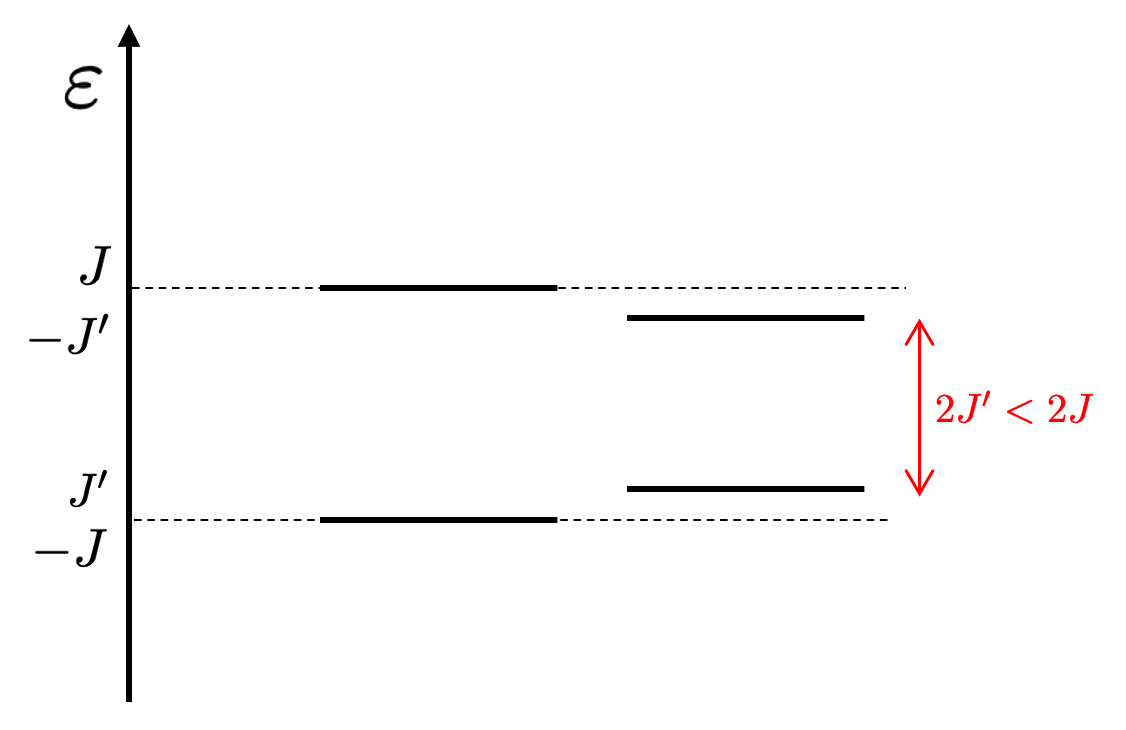
\includegraphics[width=0.58\linewidth]{images/Qubit_with_drive_1.png}
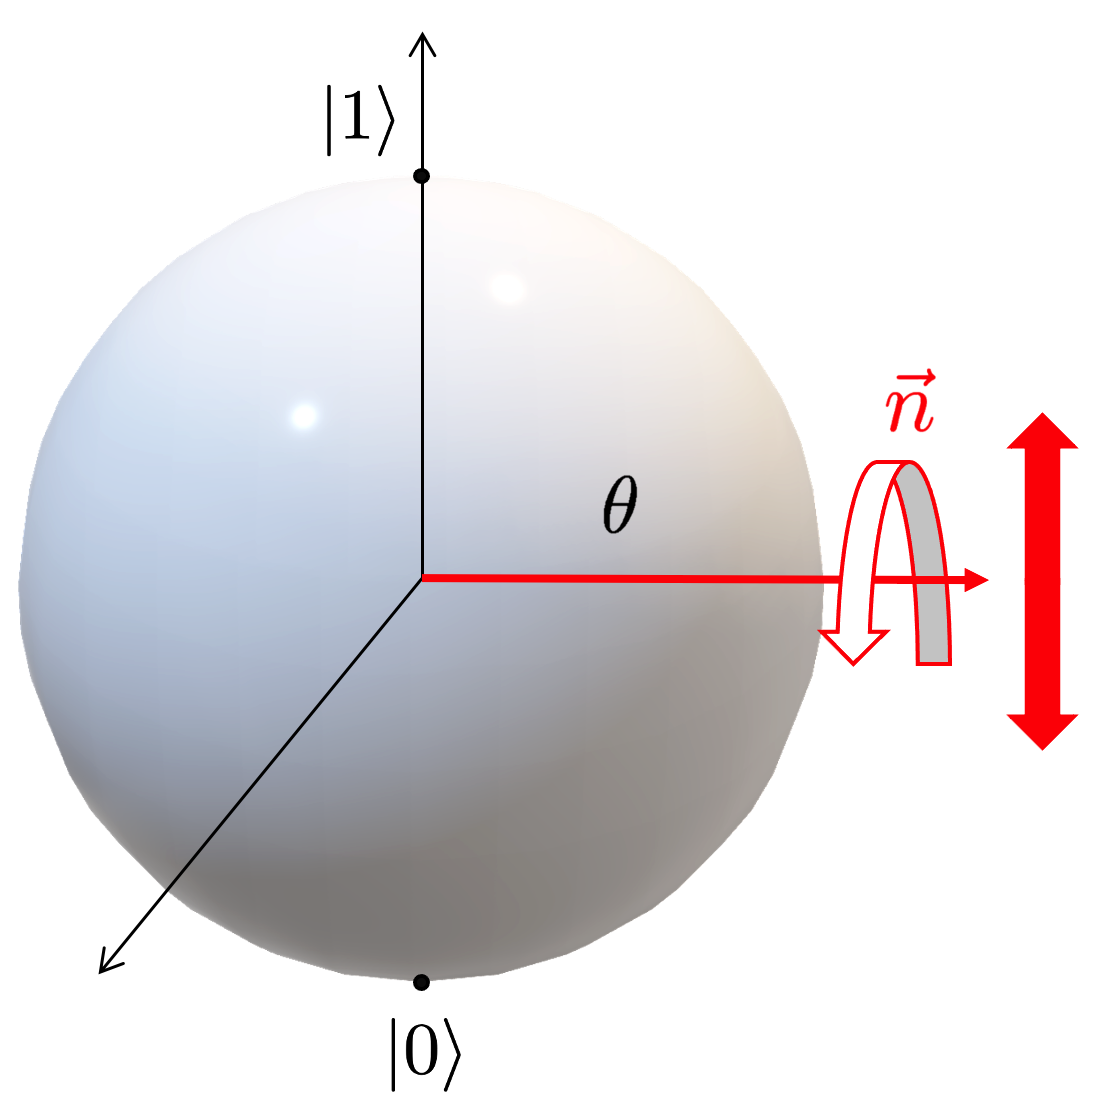
\includegraphics[width=0.37\linewidth]{images/Qubit_with_drive_2.png}
    \caption{Qubit with time periodic external potential. The system can be visualized also with a Bloch sphere which rotates around the red axis $\Vec{n}$ and which moves up and down.}
    \label{fig:quibit_drive}
\end{figure}

\begin{tcolorbox}[breakable, enhanced]
\textbf{Qubit system with a \textit{strong drive} in the high-frequency regime} \\
The aim is to study again the two-level system with the Hamiltonian (\ref{eq:qubit_H0}) and with the drive (\ref{eq:qubit_W}) but in the case in which $\hbar \omega \approx \Delta$ (strong drive).

To find the solution, one needs to reformulate the problem performing two steps: 
\begin{enumerate}
    \item $W(t)$ is removed by means of an exact unitary transformation (without expression (\ref{eq:final_ham}) and (\ref{eq:K}));
    \item another high-frequency expansion is done in the new frame (this can be done remembering that $\omega \gg J/\hbar$ is valid). 
\end{enumerate}
Summarizing, the procedure is
\begin{align*}
    \ket{\psi} \quad \xrightarrow[\text{exactly}]{R(t)} \quad \ket{\psi'} \quad \xrightarrow [\text{perturbatively}]{R'(t)} \quad \ket{\psi''}.
\end{align*}
For the first part, the transformation
\begin{align*}
    R(t) = e^{i K(t)} = \exp{i \frac{\Delta}{\hbar \omega} \sin{(\omega t)} \sigma^z}
\end{align*}
is used to obtain $H'(t)$ from (\ref{eq:Hprim}):
\begin{align*}
    R(t) H(t) R^\dagger(t) &= R(t) (H_0 + W(t)) ) R^\dagger(t) = \\
    &= R(t) H_0 R^\dagger(t) + R(t) W(t) R^\dagger(t) = \\
    &= R(t) H_0 R^\dagger(t) + W(t), \\
    \frac{dR^\dagger(t)}{dt} &= i \frac{\Delta}{\omega} \cos{(\omega t)} \omega \sigma^z \exp{-i\frac{\Delta}{\hbar \omega} \sin{(\omega t)} \sigma^z}, \\
    R(t) \frac{dR^\dagger(t)}{dt} &= -i\frac{\Delta}{\hbar} \cos{(\omega t)} R(t) \sigma^z R^\dagger(t) = \\
    &= \frac{\Delta}{\hbar} \cos{(\omega t)} \sigma^z,
\end{align*}
where it is exploited the fact that $[R(t),W(t)] = 0$ since both $R(t)$ and $W(t)$ are functions of $\sigma^z$. Therefore, 
\begin{align*}
    H'(t) &= R(t) H_0 R^\dagger(t) + W(t) - \Delta \cos{(\omega t)} \sigma^z = \\
    &= R(t) H_0 R^\dagger(t) = \\
    &= \exp{i \frac{\Delta}{\hbar \omega} \sin{(\omega t)} \sigma^z} H_0 \exp{-i \frac{\Delta}{\hbar \omega} \sin{(\omega t)} \sigma^z}
\end{align*}
The periodic potential is not present in $H'(t)$. \\
For the second part, $H'(t)$ must be rewritten in the form $H'(t) = H_0' + W'(t)$; in order to obtain this, consider the transformation $R(t)$ written as:
\begin{align*}
    R(t) = e^{i \theta (\Vec{n} \cdot \Vec{\sigma})} = \mathbb{I} \cos{\theta} + i (\Vec{n} \cdot \Vec{\sigma}) \sin{\theta} 
\end{align*}
with 
\begin{align*}
    \theta = \frac{\Delta}{\hbar \omega} \sin{(\omega t)}, \qquad \Vec{n} = \begin{pmatrix} 0 \\ 0 \\ 1 \end{pmatrix}, \qquad \text{and} \qquad \Vec{\sigma} = \begin{pmatrix} \sigma^x \\ \sigma^y \\ \sigma^z \end{pmatrix}.
\end{align*}
Remembering that $H_0 = -J \sigma^x = -J \, (\ket{0}\bra{1} + \ket{1}\bra{0})$, $H'(t)$ becomes 
\begin{align*}
    H'(t) &= R(t) H_0 R^\dagger(t) = \\
    &=- J \,  R(t)\, (\ket{0}\bra{1}) \, R^\dagger(t) - J \,  R(t)\, (\ket{1}\bra{0}) \, R^\dagger(t) = \\
    &= -J \, e^{2 i \theta}\, (\ket{0}\bra{1}) + \text{h.c.} \\
    &= -J \, \exp{2 i \frac{\Delta}{\hbar \omega} \sin{(\omega t)}}\, (\ket{0}\bra{1}) + \text{h.c.} \\
    &\equiv -J'(t)\, (\ket{0}\bra{1}) \, + \text{h.c.} 
\end{align*}
A Fourier decomposition of $J'(t)$ is allowed because one can always write 
\begin{align*}
    e^{i \alpha \sin(z)} = \sum_{n = -\infty}^{+\infty} \mathcal{J}_n(\alpha) \, e^{i n z},
\end{align*}
where $\mathcal{J}_n(\alpha)$ is a \textit{Bessel function} of the first kind at order $n$. In this case, $\alpha = 2 \Delta / (\hbar \omega)$ and $z = \omega t$; hence
\begin{align*}
    H'(t) &= -J \sum_{n = -\infty}^{+\infty} \mathcal{J}_n\left( \frac{2 \Delta}{\hbar \omega} \right) (\ket{0}\bra{1})\, e^{i n \omega t} + \text{h.c.} = \\
    &= -J \mathcal{J}_0 \left( \frac{2 \Delta}{\hbar \omega} \right) (\ket{0}\bra{1}) -J \sum\limits_{\substack{n=-\infty \\ n\neq 0}}^{+\infty} \mathcal{J}_n\left( \frac{2 \Delta}{\hbar \omega} \right) (\ket{0}\bra{1}) \, e^{i n \omega t} + \text{h.c.} = \\
     &= -J \mathcal{J}_0 \left( \frac{2 \Delta}{\hbar \omega} \right) \sigma^x -J \sum\limits_{\substack{n=-\infty \\ n\neq 0}}^{+\infty} \mathcal{J}_n\left( \frac{2 \Delta}{\hbar \omega} \right) (\ket{0}\bra{1}) \, e^{i n \omega t} + \text{h.c. ($n \neq 0$)} = \\
     &\equiv H_0' + W'(t). 
\end{align*}
Therefore, in this new frame, $H'(t)$ can be written in the form $H_0' + W'(t)$, where $H_0'$ is time-independent and $W'(t)$ represents a multi-frequency periodic part with general term which can be written as $V_n \, e^{i n \omega t}$. The expression is equivalent to (\ref{eq:start_ham}) and another perturbative approach in $\omega \gg J/\hbar$ allows to obtain an expression for the new Hamiltonian similar to (\ref{eq:final_ham}): 
\begin{align}
    H''(t) = H_0' + \frac{1}{\hbar \omega} \sum_{n,m= -\infty}^{+\infty} [V_n',V_m']  + O\left( \frac{1}{\omega^2}\right) \simeq - J \mathcal{J}_0\left( \frac{2 \Delta}{\hbar \omega} \right) \sigma^x, 
\end{align}
where the approximation at the end is done since $\omega \gg J/\hbar$ and $V_n'$ is proportional to $J$. Notice that $\Delta/(\hbar \omega)$ is a quantity without constrains and hence it could also be also $\hbar \omega \approx \Delta $. 

A final note is about the fact that for $\hbar \omega \gg \Delta$ one can write
\begin{align*}
    \mathcal{J}_0 \left( \frac{2 \Delta}{\hbar \omega} \right) \simeq 1 - \frac{1}{4}\left( \frac{2 \Delta}{\hbar \omega} \right)^4 = 1 - \frac{\Delta^2}{(\hbar \omega)^2}, 
\end{align*}
from which 
\begin{align*}
    H''(t) = -J \left(  1 - \frac{\Delta^2}{(\hbar \omega)^2} \right) \sigma^x.
\end{align*}
This result is the same obtained in the case of a weak regime. 
\end{tcolorbox}






